\documentclass{beamer}

\mode<presentation>
{
  \usetheme{Madrid}      % or try Darmstadt, Madrid, Warsaw, ...
  \usecolortheme{default} % or try albatross, beaver, crane, ...
  \usefonttheme{professionalfonts}  % or try serif, structurebold, ...
  \setbeamertemplate{navigation symbols}{}
  \setbeamertemplate{caption}[numbered]
} 

\usepackage[english]{babel}
\usepackage[utf8]{inputenc}
\usepackage[T1]{fontenc}

\title[presentation]{DESCRIPTION OF THE WOBBLING MOTION THROUGH A BOSON METHOD}
\author{Robert Poenaru}
\institute{DFT, IFIN-HH\\Doctoral School of Physics, UB}
\date{\today}

\begin{document}

\begin{frame}
  \titlepage
\end{frame}

\begin{frame}{Outline}
 \tableofcontents
\end{frame}

\section{Introduction}

\begin{frame}
  \frametitle{Nuclear Deformation}

  \begin{exampleblock}{Nuclear Radius}
    The \textbf{shape} of the nucleus is most generally described in terms of the \emph{nuclear radius}:
    \begin{align}
      R(\theta,\varphi;t)=R_0\left(1+\sum_{\lambda=0}^{^\infty}\sum_{\mu=-\lambda}^\lambda\alpha_{\lambda\mu}(t)Y_\lambda^\mu(\theta,\varphi)\right)
    \end{align}
  \end{exampleblock}
\begin{itemize}
  \item The $\alpha_{\lambda\mu}$ are collective coordinates $\Longrightarrow$ \emph{vibrations of the nucleus}.
  \item $Y_\lambda^\mu$ are the spherical harmonics.
\end{itemize}
\end{frame}


\begin{frame}{Nuclear shapes}
  Most nuclei are spherical or axially symmetric in the ground state.
    \begin{figure}
      \centering
      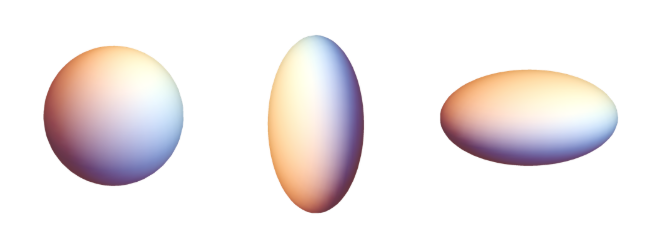
\includegraphics[scale=0.4]{figures/nuclear_shapes.png}
      \caption{\textbf{Spherical:} $\beta_2=0$ ; \textbf{Prolate:} $\beta_2>0$ ; \textbf{Oblate:} $\beta_2<0$}
    \end{figure}
  \end{frame}

\begin{frame}
  \frametitle{Quadrupole deformations}
  \begin{itemize}
    \item Most relevant vibrational degrees of freedom in nuclei.
    \item Play a crucial role in the rotational spectra of nuclei.
  \end{itemize}
\begin{block}{Quadrupole radius}
  For pure quadrupole deformations:
  \begin{align}
    R(\theta,\varphi)=R_0\left(1+\sum_\mu\alpha_{2\mu}Y_2^\mu(\theta,\varphi)\right)\ ,
  \end{align}
  Using A. Bohr's description, the coordinates $\alpha_{2\mu}$ can be reduced to only two \emph{deformation parameters}: $\beta_2$ (\emph{eccentricity}) and $\gamma$ (\textbf{triaxiality}).
\end{block}
\end{frame}

\section{Triaxial Shapes}

\begin{frame}
  \frametitle{Nuclear triaxiality}
\begin{itemize}
  \item Besides the axially symmetric shapes (i.e., spherical, prolate, and oblate), nuclei can be \textbf{triaxial} $\Longrightarrow$ lack of symmetry along any of the principal axes.
  \item The asymmetry is given by the non-zero value of $\gamma$.
\end{itemize}
\begin{figure}
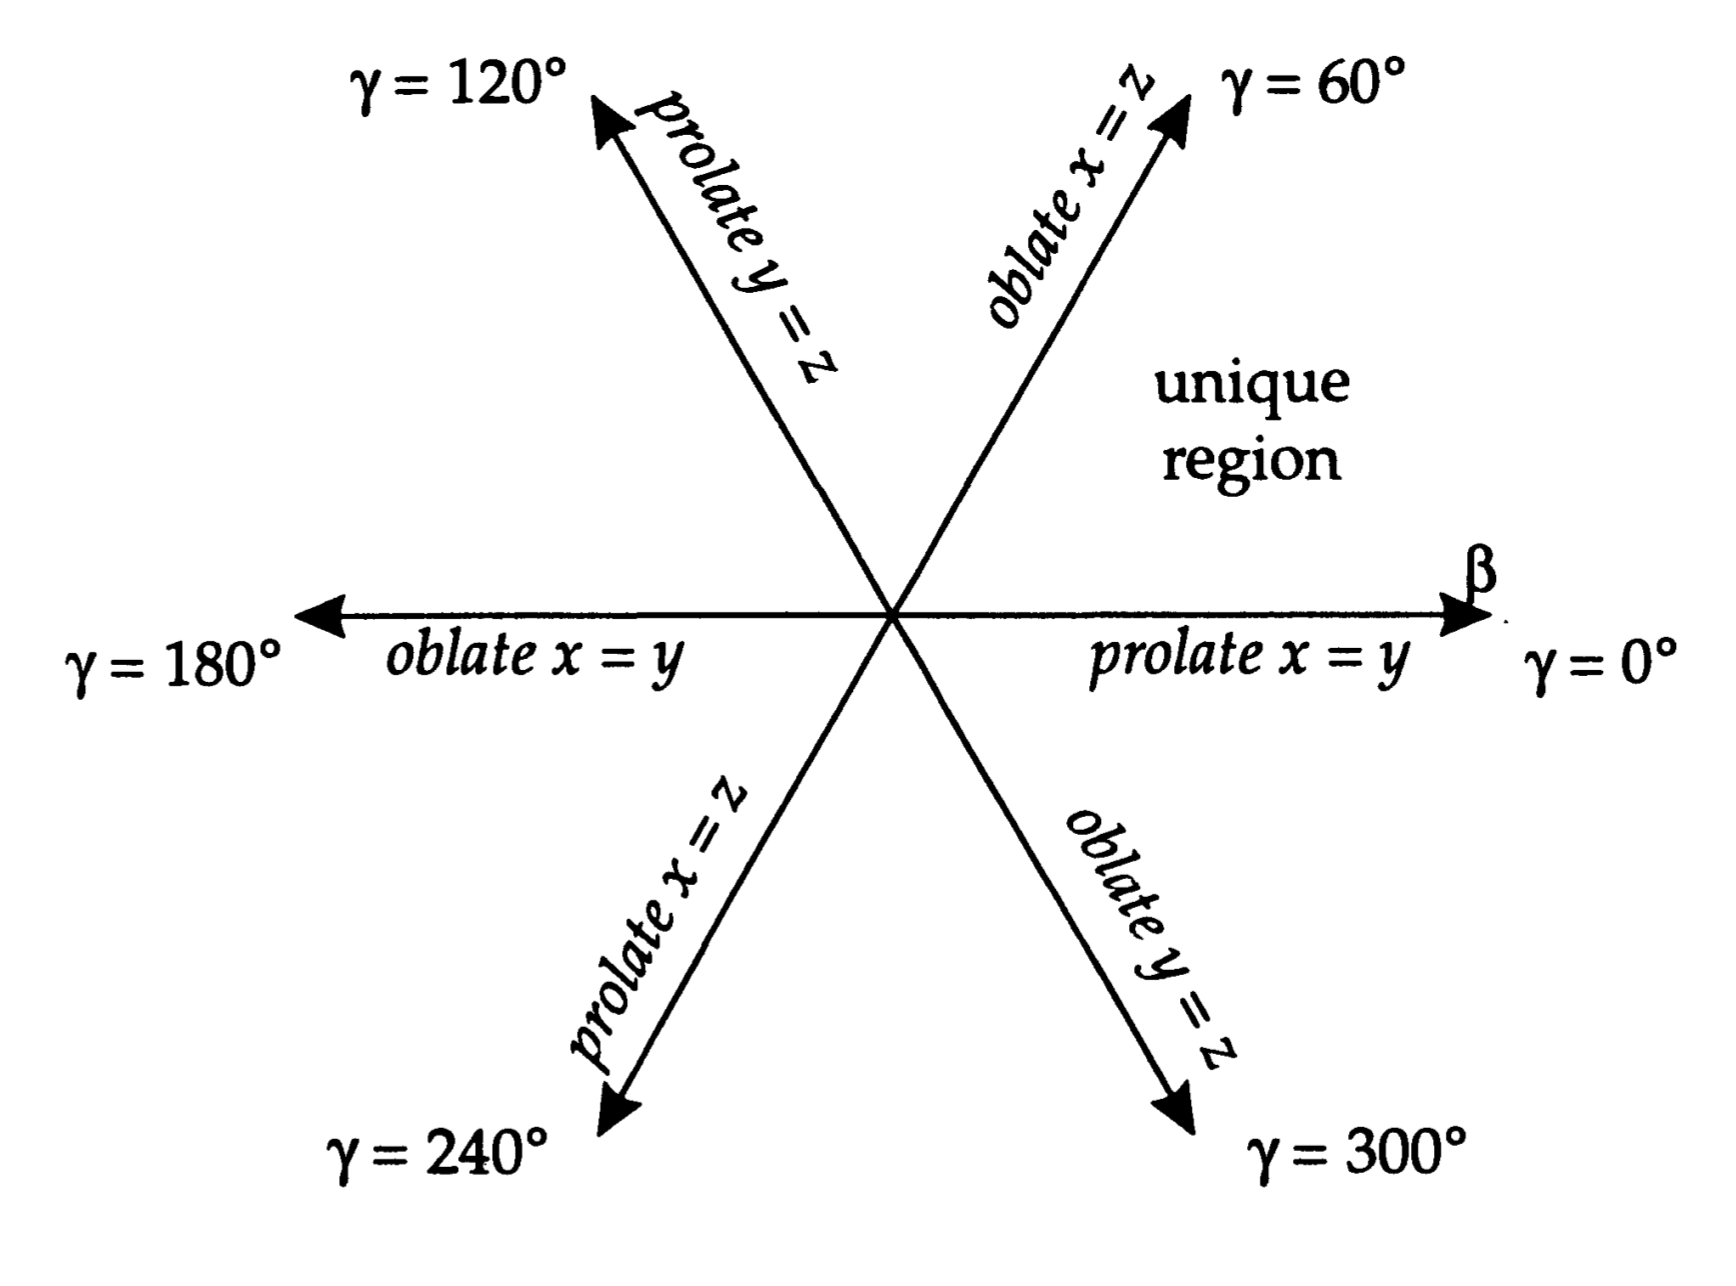
\includegraphics[scale=0.25]{figures/beta-gamma-plane.png}  
\end{figure}
\end{frame}

\begin{frame}
  \frametitle{Triaxial ellpsoid}
  \begin{figure}
    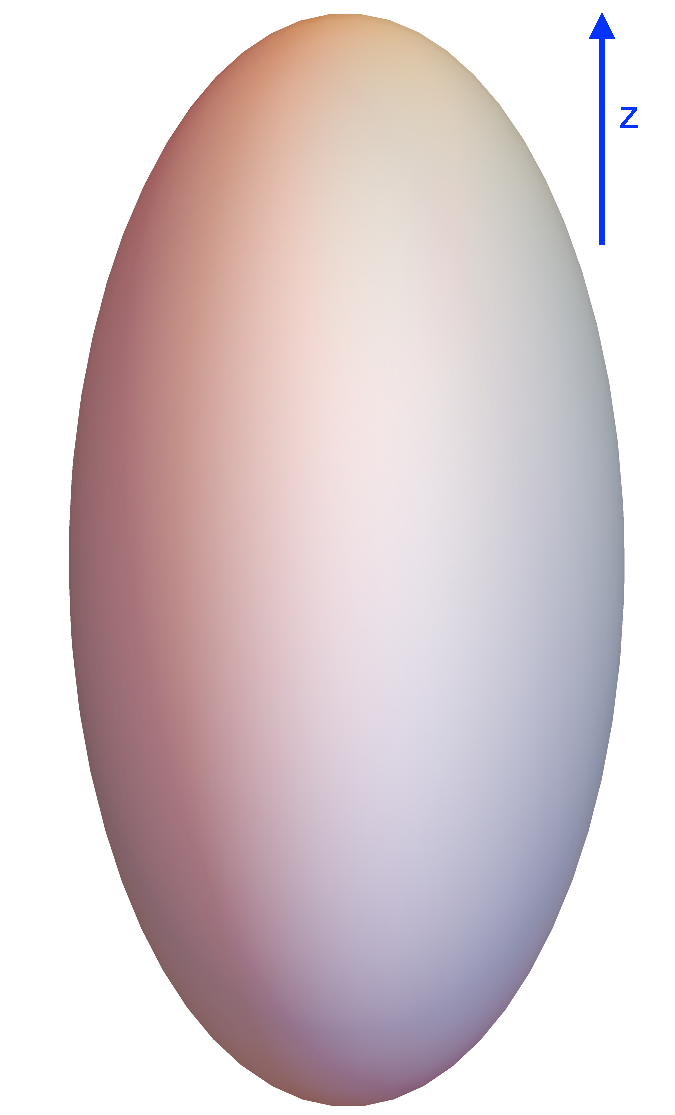
\includegraphics[scale=0.3]{figures/ellipsoid-side-view.pdf}
    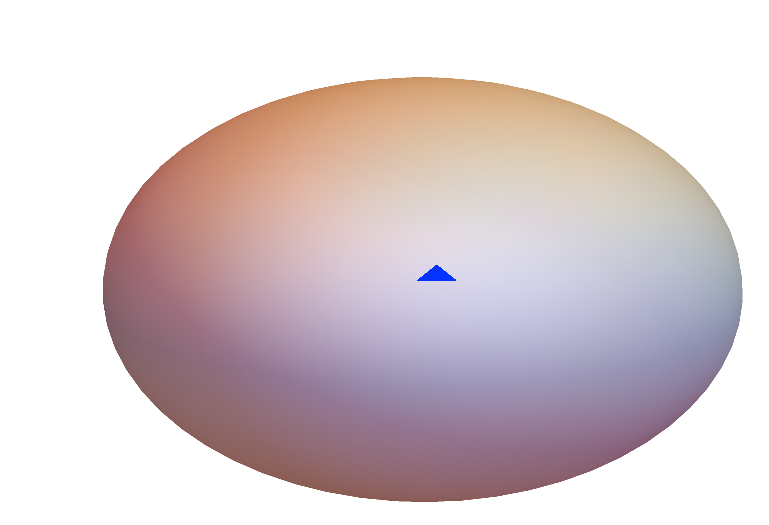
\includegraphics[scale=0.3]{figures/ellipsoid-top-view.pdf}
    \caption{\textbf{Left:} side-view\textbf{Right:} top view}
  \end{figure}

\end{frame}

\end{document}
